\documentclass[11pt,letterpaper]{article}

\usepackage[margin=2.15cm]{geometry}
\usepackage{amsmath}
\usepackage{array}
\usepackage{booktabs}
\usepackage{graphicx}
\usepackage{longtable}
\usepackage{pdflscape}
\usepackage{float}
\usepackage[hidelinks]{hyperref}

\newcommand{\ohm}{\Omega}
\newcommand{\kohm}{\text{k}\Omega}
\newcommand{\Mohm}{\text{M}\Omega}

\title{Memoria tecnica por etapas\\Sintetizador de formas de onda con LTspice}
\author{Daniel Gerardo Madriz Chavarria C24478\\
Fabricio Torres Jimenez C27803\\
Kenneth Daniel Vizcaino Jimenez C09331}
\date{I ciclo 2026}

\begin{document}

\maketitle

\section*{Resumen}

Este documento describe el diseno del sintetizador de ondas implementado en
LTspice. Se explica cada etapa, el motivo de uso de resistencias,
capacitores, transistores y flip-flop, y el calculo de los valores usados.
Tambien se comparan los valores teoricos contra los resultados simulados y se
incluyen las graficas obtenidas desde LTspice.

\section{Datos base del proyecto}

Los digitos usados para el diseno son:

\[
X=2,\qquad Y=2,\qquad Z=9.
\]

La frecuencia base se define como:

\[
f_0=\left(X+\frac{Y}{10}+\frac{Z}{100}\right)1000.
\]

Sustituyendo:

\[
f_0=\left(2+\frac{2}{10}+\frac{9}{100}\right)1000
=2290~\text{Hz}.
\]

Por tanto, las frecuencias objetivo son:

\[
f_{SC}=f_0=2290~\text{Hz},
\qquad
f_{DS}=2f_0=4580~\text{Hz},
\qquad
f_{TRI}=f_{SEN}=\frac{f_0}{2}=1145~\text{Hz}.
\]

Como \(Z=9\), el filtro seleccionado es Chebyshev tipo I de orden 5. Para la
frecuencia de corte se usa:

\[
f_c=1.25f_{TRI}=1.25(1145)=1431.25~\text{Hz}.
\]

\subsection*{Abreviaturas usadas}

Para mantener el mismo criterio en el documento, las etiquetas del esquema y
la graficadora de LTspice, se usan las siguientes abreviaturas:

\begin{center}
\begin{tabular}{ll}
\toprule
Abreviatura & Significado \\
\midrule
\(SC\) & Senal cuadrada principal del \texttt{NE555}. \\
\(VC555\) & Voltaje del capacitor de temporizacion del \texttt{NE555}. \\
\(RST\_DS\) & Pulso de reset del diente de sierra. \\
\(DS\) & Onda diente de sierra. \\
\(SC\_D2\) & Senal cuadrada dividida entre 2 por el flip-flop. \\
\(TRI\) & Onda triangular. \\
\(SEN\) & Onda senoidal filtrada. \\
\bottomrule
\end{tabular}
\end{center}

\begin{landscape}
\section{Esquema resumido del sistema}
\begin{center}
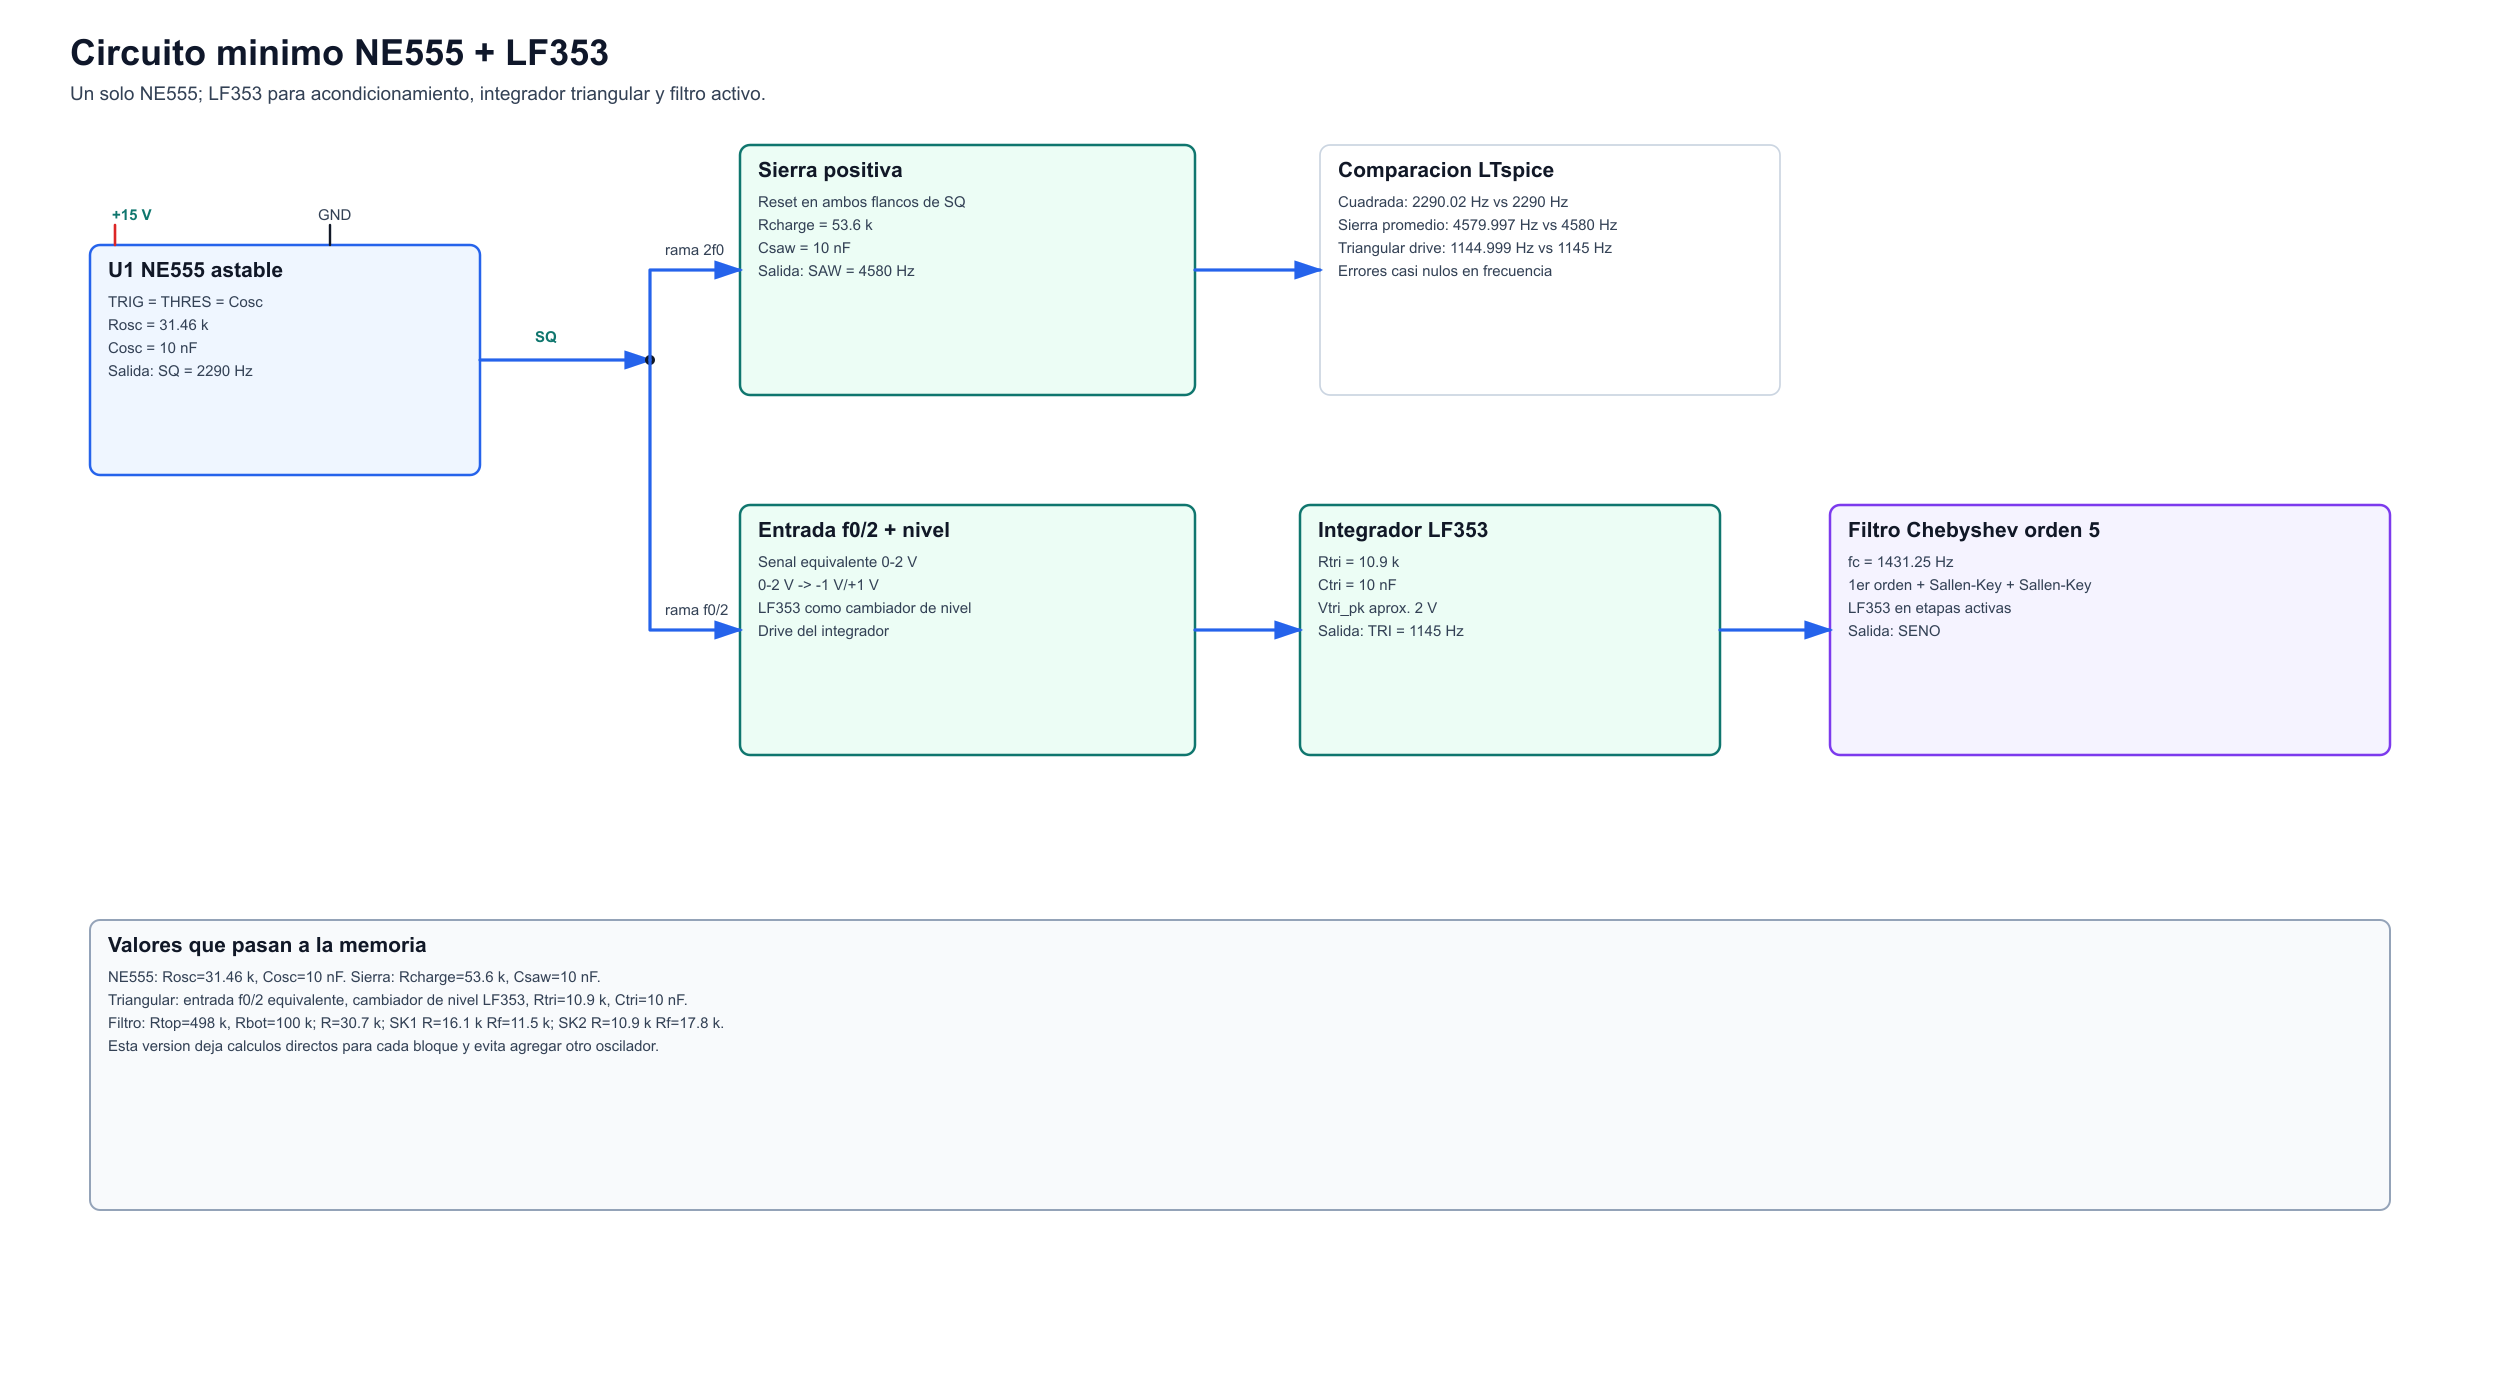
\includegraphics[width=\linewidth,height=0.82\textheight,keepaspectratio]{figuras/esquematico_minimo_ne555_lf353.png}
\end{center}
\end{landscape}

\section{Etapa 1: oscilador de onda cuadrada}

\subsection{Funcion de la etapa}

La primera etapa genera la onda cuadrada principal \(SC\). Se usa un
\texttt{NE555} porque internamente posee comparadores, un latch y una etapa de
descarga, lo cual permite construir un oscilador astable con pocos
componentes. La salida esperada es una onda cuadrada de aproximadamente
\(2290~\text{Hz}\).

\subsection{Componentes usados}

\begin{longtable}{p{2.0cm}p{4.2cm}p{8.7cm}}
\toprule
Componente & Valor & Justificacion \\
\midrule
\endhead
U1 & \texttt{NE555} & Genera la temporizacion base. Sus umbrales internos
estan cerca de \(V_{CC}/3\) y \(2V_{CC}/3\), por eso es apropiado para una
oscilacion RC estable. \\
R1 & \(31.45~\kohm\) & Resistencia de carga y descarga del capacitor de
temporizacion. Fija la frecuencia de la onda cuadrada. \\
C1 & \(10~\text{nF}\) & Capacitor de temporizacion. Se escoge \(10~\text{nF}\)
porque da una resistencia en el rango de decenas de \(\kohm\), facil de
implementar. \\
C2 & \(10~\text{nF}\) & Capacitor del pin de control del \texttt{NE555}. Reduce
ruido en los umbrales internos y estabiliza la conmutacion. \\
V1 & \(+15~\text{V}\) & Alimentacion positiva del circuito. \\
V2 & \(-15~\text{V}\) & Alimentacion negativa usada por los amplificadores
operacionales de etapas posteriores. \\
\bottomrule
\end{longtable}

\subsection{Calculo de R1 y C1}

El capacitor del \texttt{NE555} conmuta entre:

\[
V_L=\frac{V_{CC}}{3},
\qquad
V_H=\frac{2V_{CC}}{3}.
\]

Para la conexion usada, la carga y descarga tienen tiempos aproximados:

\[
t_H=R_1C_1\ln(2),
\qquad
t_L=R_1C_1\ln(2).
\]

Entonces:

\[
T=t_H+t_L=2R_1C_1\ln(2).
\]

\[
f_0=\frac{1}{2R_1C_1\ln(2)}.
\]

Despejando:

\[
R_1=\frac{1}{2f_0C_1\ln(2)}.
\]

Con \(C_1=10~\text{nF}\) se selecciona:

\[
\boxed{R_1=31.45~\kohm}
\]

Este valor se usa tanto en el calculo final como en la simulacion. Al
sustituirlo en el modelo ideal de temporizacion:

\[
f_{SC,calc}=
\frac{1}{2(31.45\times10^3)(10\times10^{-9})\ln(2)}
=2293.63~\text{Hz}.
\]

La simulacion con el modelo del \texttt{NE555} entrega
\(2289.8233~\text{Hz}\), que es el valor reportado en la validacion.

\section{Etapa 2: diente de sierra positivo}

\subsection{Funcion de la etapa}

La segunda etapa convierte la onda cuadrada \(SC\) en una onda diente de
sierra \(DS\). El capacitor \(C4\) se carga lentamente mediante \(R6\), y se
descarga rapidamente con el transistor \(Q1\). Para obtener una sierra a
\(2f_0\), el capacitor se descarga tanto en el flanco de subida como en el
flanco de bajada de \(SC\).

\subsection{Componentes usados}

\begin{longtable}{p{2.0cm}p{4.2cm}p{8.7cm}}
\toprule
Componente & Valor & Justificacion \\
\midrule
\endhead
C4 & \(10~\text{nF}\) & Capacitor principal de la rampa. Su voltaje es la onda
diente de sierra. \\
R6 & \(53.6~\kohm\) & Carga \(C4\) desde \(+15~\text{V}\). Su valor determina
la pendiente de la rampa y la amplitud de \(DS\). \\
Q1 & \texttt{2N3904} & Transistor de descarga. Al recibir un pulso en la base,
descarga rapidamente \(C4\) a tierra. \\
R5 & \(3.3~\kohm\) & Limita la corriente de base de \(Q1\). Protege el
transistor y asegura saturacion durante el reset. \\
R4 & \(47~\kohm\) & Pull-down de la base de \(Q1\). Mantiene el transistor
apagado cuando no hay pulso de reset. \\
C3 & \(1~\text{nF}\) & Capacitor de acople para detectar un flanco de \(SC\).
Forma un pulso corto con \(R2\). \\
R2 & \(10~\kohm\) & Descarga \(C3\) y fija el ancho aproximado del pulso:
\(\tau=R2C3=10~\mu\text{s}\). \\
D1 & \texttt{1N4148} & Diodo rapido que suma el pulso de un flanco hacia el
nodo \texttt{RST\_DS} sin devolver corriente a la rama anterior. \\
Q2 & \texttt{2N3904} & Inversor de la onda cuadrada. Permite detectar el otro
flanco de \(SC\). \\
R7 & \(47~\kohm\) & Resistencia de entrada a la base de \(Q2\). Limita la
corriente de base. \\
R8 & \(100~\kohm\) & Descarga la base de \(Q2\) y define un estado bajo
seguro cuando \(SC\) esta bajo. \\
R9 & \(10~\kohm\) & Pull-up del colector de \(Q2\). Genera la senal invertida
con nivel alto cuando \(Q2\) esta apagado. \\
C5 & \(1~\text{nF}\) & Capacitor de acople para el flanco de la senal
invertida. \\
R10 & \(10~\kohm\) & Descarga \(C5\) y fija otro pulso de aproximadamente
\(10~\mu\text{s}\). \\
D2 & \texttt{1N4148} & Suma el pulso de la rama invertida al nodo
\texttt{RST\_DS}. \\
R3 & \(47~\kohm\) & Pull-down del nodo \texttt{RST\_DS}. Mantiene ese nodo
en cero cuando no hay pulsos. \\
\bottomrule
\end{longtable}

\subsection{Calculo de R6 y C4}

Como se descarga en ambos flancos:

\[
f_{DS}=2f_0=4580~\text{Hz}.
\]

Por tanto:

\[
T_{DS}=\frac{1}{2f_0}
=\frac{1}{4580}
=218.34~\mu\text{s}.
\]

La carga del capacitor sigue:

\[
v_C(t)=V_{CC}\left(1-e^{-t/(R6C4)}\right).
\]

Se desea una rampa cercana a \(5~\text{V}\), con \(V_{CC}=15~\text{V}\):

\[
V_{DS,pk}=V_{CC}\left(1-e^{-T_{DS}/(R6C4)}\right).
\]

Despejando:

\[
R6=
\frac{-T_{DS}}
{C4\ln\left(1-\frac{V_{DS,pk}}{V_{CC}}\right)}.
\]

Con \(C4=10~\text{nF}\):

\[
R6=
\frac{-218.34\times10^{-6}}
{(10\times10^{-9})\ln\left(1-\frac{5}{15}\right)}
=53.85~\kohm.
\]

Se usa:

\[
\boxed{R6=53.6~\kohm}.
\]

\subsection{Ancho de los pulsos de reset}

Las ramas \(C3\)-\(R2\) y \(C5\)-\(R10\) son detectores de flanco. Su constante
de tiempo es:

\[
\tau=(10~\kohm)(1~\text{nF})=10~\mu\text{s}.
\]

Este valor es mucho menor que \(T_{DS}=218.34~\mu\text{s}\), por lo que el
pulso solo descarga el capacitor y no destruye la rampa.

\section{Etapa 3: divisor por 2 e integrador triangular}

\subsection{Funcion de la etapa}

La etapa 3 produce una onda triangular \(TRI\) a \(f_0/2\). Primero se usa un
flip-flop tipo D \texttt{CD4013B} para dividir la frecuencia de \(SC\) entre 2.
Luego esa salida se aplica a un integrador con \texttt{LF353}.

\subsection{Flip-flop divisor por 2}

\begin{longtable}{p{2.0cm}p{4.2cm}p{8.7cm}}
\toprule
Componente & Valor & Justificacion \\
\midrule
\endhead
U2 & \texttt{CD4013B} & Flip-flop D. Se conecta la salida negada a la entrada
D, de modo que el estado cambia en cada flanco de reloj. Asi se divide la
frecuencia entre 2. \\
\texttt{CLK} & \(SC\) & La onda cuadrada principal sirve como reloj del
flip-flop. \\
\texttt{Q} & \(SC\_D2\) & Salida dividida. Su frecuencia objetivo es
\(1145~\text{Hz}\). \\
\texttt{S}, \texttt{R} & \(0~\text{V}\) & Set y reset se dejan inactivos para
que el flip-flop funcione como divisor. \\
\bottomrule
\end{longtable}

\subsection{Integrador triangular}

\begin{longtable}{p{2.0cm}p{4.2cm}p{8.7cm}}
\toprule
Componente & Valor & Justificacion \\
\midrule
\endhead
U3 & \texttt{LF353} & Amplificador operacional JFET. Se usa como integrador
inversor por su alta impedancia de entrada y buena velocidad para estas
frecuencias. \\
R11 & \(27.4~\kohm\) & Resistencia de entrada del integrador. Fija la
pendiente de la triangular junto con \(C6\). \\
R12 & \(168~\kohm\) & Resistencia hacia \(-15~\text{V}\). Introduce una
corriente de compensacion para centrar la salida del integrador. \\
C6 & \(10~\text{nF}\) & Capacitor de realimentacion. Convierte la corriente de
entrada en una pendiente lineal de voltaje. \\
R13 & \(1~\Mohm\) & Resistencia de fuga en paralelo con \(C6\). Evita que el
integrador se sature por offset DC y acelera el asentamiento sin afectar mucho
la senal de \(1145~\text{Hz}\). \\
\bottomrule
\end{longtable}

\subsection{Calculo de R11}

La salida \(SC\_D2\) esta aproximadamente entre \(0~\text{V}\) y
\(5~\text{V}\). Luego de centrarla, su componente alterna es de
aproximadamente:

\[
V_{drv}\approx 2.5~\text{V}.
\]

Para un integrador:

\[
\frac{dv_o}{dt}=-\frac{v_i}{R11C6}.
\]

Durante medio periodo de la triangular, la salida debe cambiar de
\(-V_{TRI,pk}\) a \(+V_{TRI,pk}\), por lo que:

\[
\Delta V=2V_{TRI,pk}.
\]

Como \(f_{TRI}=f_0/2\), el medio periodo de \(TRI\) es:

\[
\frac{1}{2f_{TRI}}=\frac{1}{f_0}.
\]

Entonces:

\[
2V_{TRI,pk}=
\frac{V_{drv}}{R11C6}\frac{1}{f_0}.
\]

Despejando:

\[
R11=
\frac{V_{drv}}{2V_{TRI,pk}f_0C6}.
\]

Con \(V_{drv}=2.5~\text{V}\), \(V_{TRI,pk}=2~\text{V}\),
\(f_0=2290~\text{Hz}\) y \(C6=10~\text{nF}\):

\[
R11=
\frac{2.5}{2(2)(2290)(10\times10^{-9})}
=27.29~\kohm.
\]

Se usa:

\[
\boxed{R11=27.4~\kohm}.
\]

\subsection{Calculo de R12}

La resistencia \(R12\) compensa la componente DC de \(SC\_D2\). En el nodo
inversor del integrador, el promedio de corriente debe ser aproximadamente
cero:

\[
\frac{\overline{V}_{SC\_D2}}{R11}
+\frac{-15}{R12}=0.
\]

Por tanto:

\[
R12=\frac{15R11}{\overline{V}_{SC\_D2}}.
\]

Como la salida del flip-flop real en LTspice queda cerca de \(0\) a
\(4.94~\text{V}\), se toma
\(\overline{V}_{SC\_D2}\approx 2.45~\text{V}\):

\[
R12=\frac{15(27.4~\kohm)}{2.45}=167.8~\kohm.
\]

Se usa:

\[
\boxed{R12=168~\kohm}.
\]

\subsection{Justificacion de R13}

Un integrador ideal no tiene camino DC en la realimentacion. En simulacion y
en la practica, cualquier offset puede hacer que la salida se vaya a
saturacion. Por eso se coloca \(R13\) en paralelo con \(C6\).

Para la frecuencia de interes:

\[
X_{C6}=\frac{1}{2\pi f_{TRI}C6}
=\frac{1}{2\pi(1145)(10~\text{nF})}
=13.9~\kohm.
\]

Como \(R13=1~\Mohm\), se cumple:

\[
R13 \gg X_{C6}.
\]

Por eso casi no modifica la integracion a \(1145~\text{Hz}\), pero si da una
ruta DC que evita saturacion y mejora la convergencia.

\section{Etapa 4: filtro pasabajas Chebyshev de orden 5}

\subsection{Funcion de la etapa}

El filtro convierte la onda triangular en una senal senoidal. Se usa la
triangular como entrada porque ya es mas suave que la cuadrada y que la
sierra: tiene menos cambios abruptos, por lo que el filtro necesita atenuar
menos contenido de alta frecuencia.

Como \(Z=9\), se selecciona Chebyshev tipo I. La ventaja de esta respuesta es
que ofrece una transicion mas rapida que Butterworth para el mismo orden,
aceptando rizado en la banda de paso.

\subsection{Estructura}

Un filtro de quinto orden se implementa como:

\[
5=1+2+2.
\]

Por tanto, se usa:

\begin{itemize}
  \item un atenuador de entrada;
  \item una etapa pasabajas de primer orden;
  \item una seccion Sallen-Key de segundo orden;
  \item una segunda seccion Sallen-Key de segundo orden.
\end{itemize}

\subsection{Coeficientes usados}

Para \(f_c=1431.25~\text{Hz}\), \(C=10~\text{nF}\) y respuesta Chebyshev de
orden 5, se usan los multiplicadores:

\[
p_1=0.3623196,
\qquad
s_1=0.6904832,
\qquad
Q_1=1.1778056,
\]

\[
s_2=1.0177347,
\qquad
Q_2=4.5449633.
\]

\subsection{Atenuador de entrada}

\begin{longtable}{p{2.0cm}p{4.2cm}p{8.7cm}}
\toprule
Componente & Valor & Justificacion \\
\midrule
\endhead
R14 & \(498~\kohm\) & Resistencia superior del divisor de entrada. Atenua la
triangular antes de las etapas activas. \\
R15 & \(100~\kohm\) & Resistencia inferior del divisor. Se escoge alta para
no cargar demasiado al integrador. \\
\bottomrule
\end{longtable}

Las etapas Sallen-Key tienen ganancias mayores que 1. Para evitar que la
salida se sature, se coloca un atenuador de entrada. Con:

\[
K_1=1+\frac{R19}{R20}=1+\frac{11.5}{10}=2.15,
\]

\[
K_2=1+\frac{R22}{R23}=1+\frac{17.8}{10}=2.78.
\]

La ganancia total aproximada es:

\[
K_1K_2=2.15(2.78)=5.98.
\]

Se escoge \(R15=100~\kohm\), y se calcula:

\[
R14=R15(K_1K_2-1).
\]

\[
R14=100~\kohm(5.98-1)=498~\kohm.
\]

\subsection{Etapa de primer orden}

\begin{longtable}{p{2.0cm}p{4.2cm}p{8.7cm}}
\toprule
Componente & Valor & Justificacion \\
\midrule
\endhead
R16 & \(30.7~\kohm\) & Resistencia del polo de primer orden. Se calcula con el
multiplicador Chebyshev \(p_1\). \\
C7 & \(10~\text{nF}\) & Capacitor del polo de primer orden. Se mantiene el
mismo valor base de capacitor para simplificar el diseno. \\
\bottomrule
\end{longtable}

\[
R16=\frac{1}{2\pi f_cp_1C7}.
\]

\[
R16=
\frac{1}{2\pi(1431.25)(0.3623196)(10~\text{nF})}
=30.7~\kohm.
\]

\subsection{Primera seccion Sallen-Key}

\begin{longtable}{p{2.0cm}p{4.2cm}p{8.7cm}}
\toprule
Componente & Valor & Justificacion \\
\midrule
\endhead
R17 & \(16.1~\kohm\) & Primera resistencia de la red Sallen-Key. \\
R18 & \(16.1~\kohm\) & Segunda resistencia de la red Sallen-Key. Se usa igual
a R17 para aplicar la formula simplificada. \\
C8 & \(10~\text{nF}\) & Capacitor de la red Sallen-Key conectado hacia la
salida de la seccion. Esta conexion es esencial para la respuesta de segundo
orden. \\
C10 & \(10~\text{nF}\) & Capacitor a tierra de la red Sallen-Key. \\
U5 & \texttt{LF353} & Amplificador no inversor de la primera seccion. \\
R19 & \(11.5~\kohm\) & Realimentacion de ganancia de U5. \\
R20 & \(10~\kohm\) & Resistencia a tierra de la red de ganancia de U5. \\
\bottomrule
\end{longtable}

Para la frecuencia de esta seccion:

\[
R17=R18=\frac{1}{2\pi f_cs_1C}.
\]

\[
R17=R18=
\frac{1}{2\pi(1431.25)(0.6904832)(10~\text{nF})}
=16.1~\kohm.
\]

La ganancia de una seccion Sallen-Key con componentes iguales se aproxima con:

\[
K=3-\frac{1}{Q}.
\]

Para \(Q_1=1.1778056\):

\[
K_1=3-\frac{1}{1.1778056}=2.151.
\]

Con \(R20=10~\kohm\):

\[
R19=(K_1-1)R20=1.151(10~\kohm)=11.5~\kohm.
\]

\subsection{Segunda seccion Sallen-Key}

\begin{longtable}{p{2.0cm}p{4.2cm}p{8.7cm}}
\toprule
Componente & Valor & Justificacion \\
\midrule
\endhead
R24 & \(10.9~\kohm\) & Primera resistencia de la segunda red Sallen-Key. \\
R21 & \(10.9~\kohm\) & Segunda resistencia de la segunda red Sallen-Key. \\
C9 & \(10~\text{nF}\) & Capacitor conectado hacia la salida final \(SEN\). \\
C11 & \(10~\text{nF}\) & Capacitor a tierra de la segunda seccion. \\
U4 & \texttt{LF353} & Amplificador no inversor de la segunda seccion. \\
R22 & \(17.8~\kohm\) & Realimentacion de ganancia de U4. \\
R23 & \(10~\kohm\) & Resistencia a tierra de la ganancia de U4. \\
\bottomrule
\end{longtable}

\[
R24=R21=\frac{1}{2\pi f_cs_2C}.
\]

\[
R24=R21=
\frac{1}{2\pi(1431.25)(1.0177347)(10~\text{nF})}
=10.9~\kohm.
\]

Para \(Q_2=4.5449633\):

\[
K_2=3-\frac{1}{4.5449633}=2.780.
\]

Con \(R23=10~\kohm\):

\[
R22=(K_2-1)R23=1.780(10~\kohm)=17.8~\kohm.
\]

\section{Comparacion de valores teoricos y simulados}

La simulacion integrada final se verifico con el esquema corregido:

\[
\texttt{entrega\_sintetizador\_ltspice/simulacion/EsquematicoSintetizador.asc}.
\]

Para regenerar los datos de forma portable tambien se uso:

\[
\texttt{entrega\_sintetizador\_ltspice/simulacion/EsquematicoSintetizador\_portable.cir}.
\]

La directiva transitoria usada fue:

\[
\texttt{.tran 0 120m 0 1u}.
\]

Ademas, el esquema guarda explicitamente las senales principales para que
aparezcan disponibles en la graficadora de LTspice:

\[
\texttt{.save V(SC) V(VC555) V(RST\_DS) V(DS) V(SC\_D2) V(TRI) V(SEN)}.
\]

El archivo \texttt{EsquematicoSintetizador.plt} se dejo con paneles separados
para \(SC\), \(VC555\), \(RST\_DS\), \(DS\), \(SC\_D2\), \(TRI\) y \(SEN\).
Al correr el esquema o abrir el \texttt{.raw}, esas son las senales que se
pueden visualizar directamente en la ventana de graficas.

\subsection{Mediciones de LTspice ordenadas por etapa}

Las siguientes tablas separan los datos que aparecen en el log de LTspice por
etapa del sintetizador. Asi se puede validar cada bloque sin mezclar las
mediciones de frecuencia, amplitud y nivel medio.

\begin{table}[H]
\centering
\begin{tabular}{lrrr}
\toprule
Parametro & Teorico & LTspice & Error [\%] \\
\midrule
Frecuencia de \(SC\) [Hz] & 2290.00 & 2289.8233 & -0.00771 \\
Ciclo de trabajo de \(SC\) [\%] & 50.00 & 50.0105 & +0.02091 \\
\(V_{pp}\) de \(SC\) [V] & -- & 14.9961 & -- \\
\(V_{pp}\) de \(VC555\) [V] & -- & 5.0060 & -- \\
\bottomrule
\end{tabular}
\caption{Resultados simulados de la etapa 1: oscilador \texttt{NE555}.}
\end{table}

Por tanto, el ciclo de trabajo validado por simulacion es:

\[
D_{SC}=50.0105\%.
\]

\begin{table}[H]
\centering
\begin{tabular}{lrrr}
\toprule
Parametro & Teorico & LTspice & Error [\%] \\
\midrule
Frecuencia de \(DS\) [Hz] & 4580.00 & 4579.3252 & -0.01473 \\
\(V_{pp}\) de \(DS\) [V] & -- & 4.8940 & -- \\
\(V_{max}\) de \(RST\_DS\) [V] & -- & 14.1075 & -- \\
\bottomrule
\end{tabular}
\caption{Resultados simulados de la etapa 2: diente de sierra.}
\end{table}

\begin{table}[H]
\centering
\begin{tabular}{lrrr}
\toprule
Parametro & Teorico & LTspice & Error [\%] \\
\midrule
Frecuencia de \(SC\_D2\) [Hz] & 1145.00 & 1144.9076 & -0.00807 \\
\(V_{pp}\) de \(SC\_D2\) [V] & -- & 4.9709 & -- \\
Frecuencia directa de \(TRI\) [Hz] & 1145.00 & 1145.9762 & +0.08526 \\
Frecuencia de referencia de \(TRI\) [Hz] & 1145.00 & 1144.9076 & -0.00807 \\
\(V_{pp}\) de \(TRI\) [V] & -- & 3.9933 & -- \\
\(\overline{V}\) de \(TRI\) [V] & -- & -0.0694 & -- \\
\bottomrule
\end{tabular}
\caption{Resultados simulados de la etapa 3: divisor por dos e integrador.}
\end{table}

\begin{table}[H]
\centering
\begin{tabular}{lrrr}
\toprule
Parametro & Teorico & LTspice & Error [\%] \\
\midrule
Frecuencia de \(SEN\) [Hz] & 1145.00 & 1144.8698 & -0.01137 \\
\(V_{pp}\) de \(SEN\) [V] & -- & 0.8762 & -- \\
\(\overline{V}\) de \(SEN\) [V] & -- & -0.0301 & -- \\
Ganancia \(V_{pp,SEN}/V_{pp,TRI}\) [V/V] & -- & 0.2194 & -- \\
\bottomrule
\end{tabular}
\caption{Resultados simulados de la etapa 4: filtro pasabajas y salida senoidal.}
\end{table}

\subsection{Frecuencias}

\begin{table}[H]
\centering
\begin{tabular}{lrrr}
\toprule
Senal & Teorico [Hz] & LTspice [Hz] & Error [\%] \\
\midrule
Cuadrada \(SC\) & 2290.00 & 2289.8233 & -0.00771 \\
Diente de sierra \(DS\) & 4580.00 & 4579.3252 & -0.01473 \\
Flip-flop \(SC\_D2\) & 1145.00 & 1144.9076 & -0.00807 \\
Triangular \(TRI\) & 1145.00 & 1145.9762 & +0.08526 \\
Senoidal \(SEN\) & 1145.00 & 1144.8698 & -0.01137 \\
\bottomrule
\end{tabular}
\caption{Comparacion de frecuencias teoricas contra LTspice.}
\end{table}

Para la triangular tambien se reporta una referencia segura:

\[
f_{TRI,ref}=f_{SC\_D2}=1144.9076~\text{Hz}.
\]

Esto se usa porque el integrador cambia la forma y el nivel de la onda, pero
no cambia el periodo impuesto por el flip-flop.

\subsection{Amplitudes y niveles medios}

\begin{table}[H]
\centering
\begin{tabular}{lrr}
\toprule
Senal & \(V_{pp}\) simulado [V] & Nivel medio simulado [V] \\
\midrule
\(SC\) & 14.9961 & -- \\
\(VC555\) & 5.0060 & -- \\
\(DS\) & 4.8940 & -- \\
\(SC\_D2\) & 4.9709 & -- \\
\(TRI\) & 3.9933 & -0.0694 \\
\(SEN\) & 0.8762 & -0.0301 \\
\bottomrule
\end{tabular}
\caption{Amplitudes obtenidas en LTspice.}
\end{table}

\section{Respuesta del filtro}

La simulacion AC del filtro entrega:

\begin{table}[H]
\centering
\begin{tabular}{lr}
\toprule
Punto de medicion & Magnitud LTspice \\
\midrule
\(|H(1145~\text{Hz})|\) & \(-11.1189~\text{dB}\) \\
\(|H(3435~\text{Hz})|\) & \(-62.2899~\text{dB}\) \\
Atenuacion adicional de la tercera armonica & \(51.1710~\text{dB}\) \\
\bottomrule
\end{tabular}
\caption{Resultados del Bode del filtro Chebyshev.}
\end{table}

\[
|H(1145~\text{Hz})|=-11.12~\text{dB}.
\]

\[
|H(3435~\text{Hz})|=-62.29~\text{dB}.
\]

La diferencia es:

\[
62.29-11.12=51.17~\text{dB}.
\]

Esto indica que una frecuencia tres veces mayor que la fundamental queda muy
atenuada respecto a la frecuencia de interes.

La corrida AC del Bode corresponde al filtro aislado con un buffer despues del
polo \(R16\)-\(C7\). El esquema integrado final conserva ese mismo buffer,
por lo que la respuesta AC representa directamente al filtro conectado en el
sintetizador completo.

\begin{figure}[H]
\centering
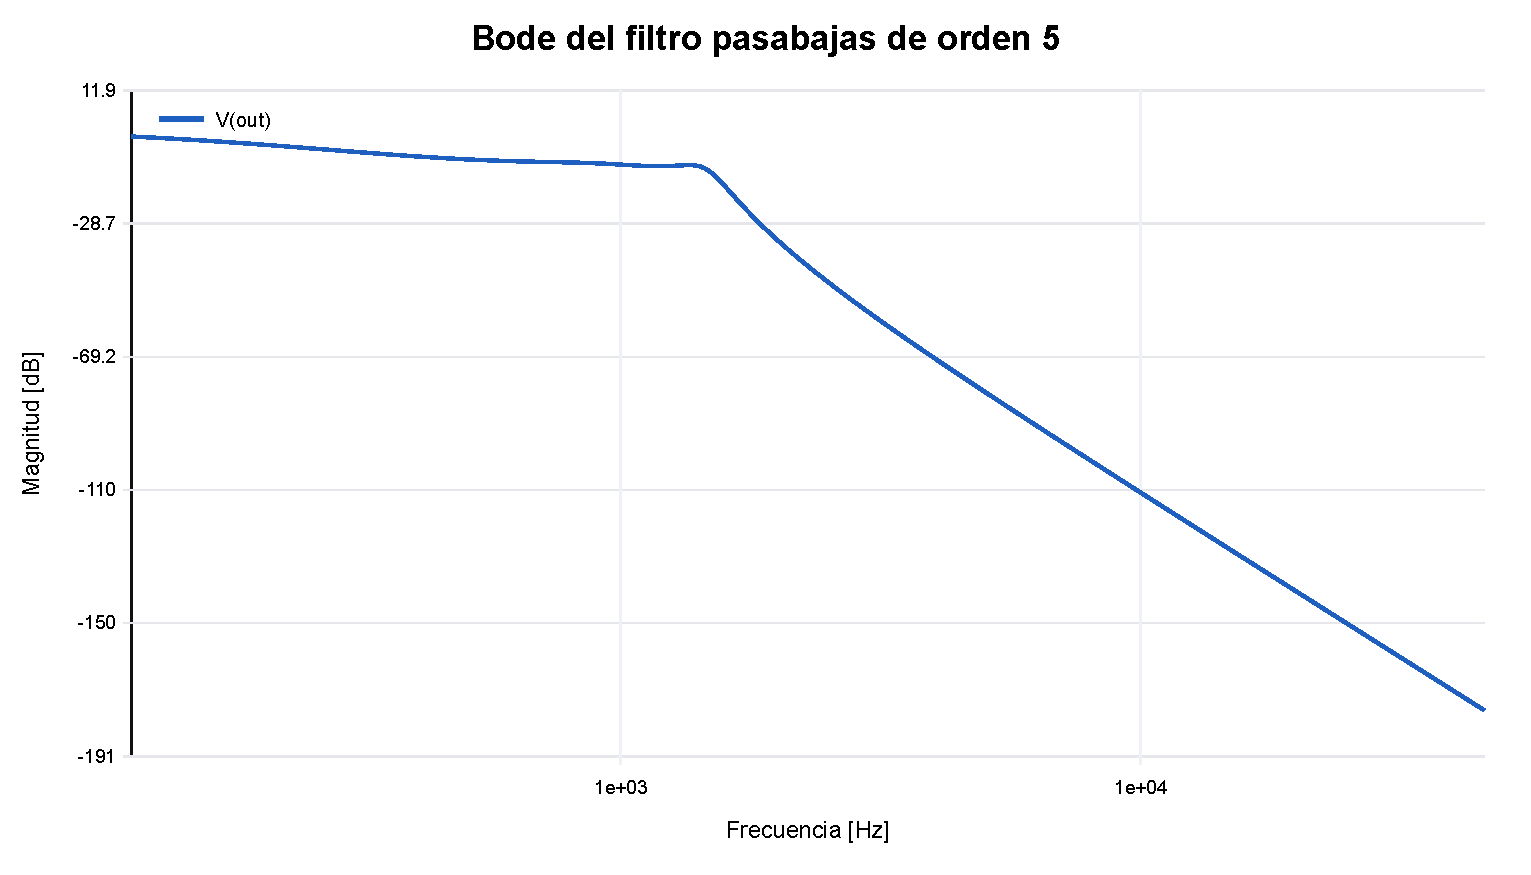
\includegraphics[width=0.92\linewidth]{figuras/integrado_bode_filtro.pdf}
\caption{Respuesta en frecuencia del filtro pasabajas.}
\end{figure}

\section{Graficas de LTspice por separado}

Las graficas siguientes se obtuvieron del archivo \texttt{.raw} del esquema
integrado corregido. Se muestran ventanas despues del asentamiento del
circuito.

\begin{figure}[H]
\centering
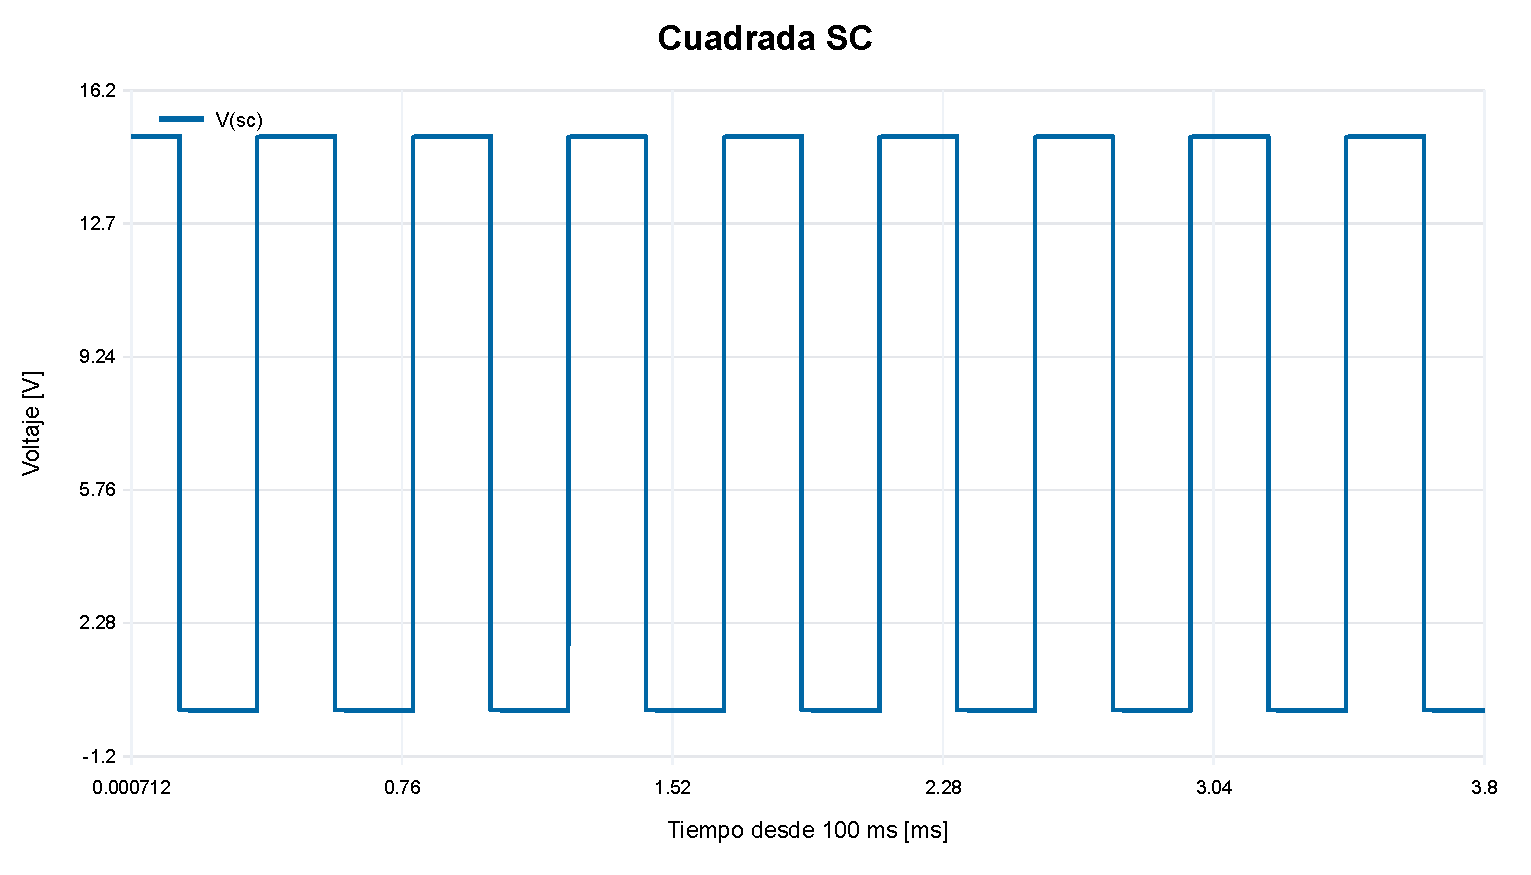
\includegraphics[width=0.88\linewidth]{figuras/integrado_sc.pdf}
\caption{Onda cuadrada \(SC\).}
\end{figure}

\begin{figure}[H]
\centering
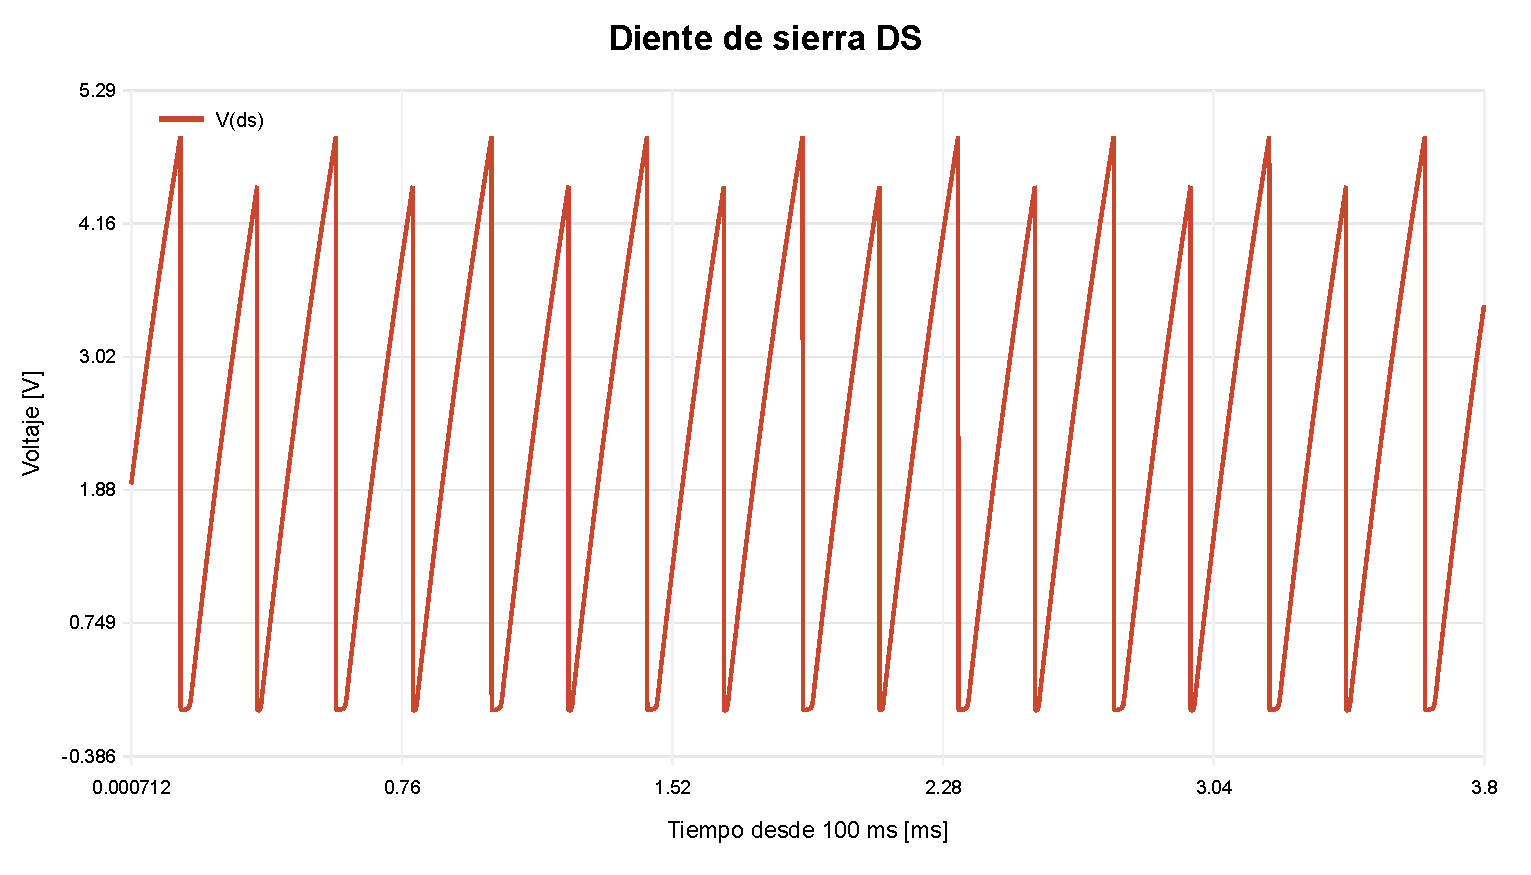
\includegraphics[width=0.88\linewidth]{figuras/integrado_ds.pdf}
\caption{Onda diente de sierra \(DS\).}
\end{figure}

\begin{figure}[H]
\centering
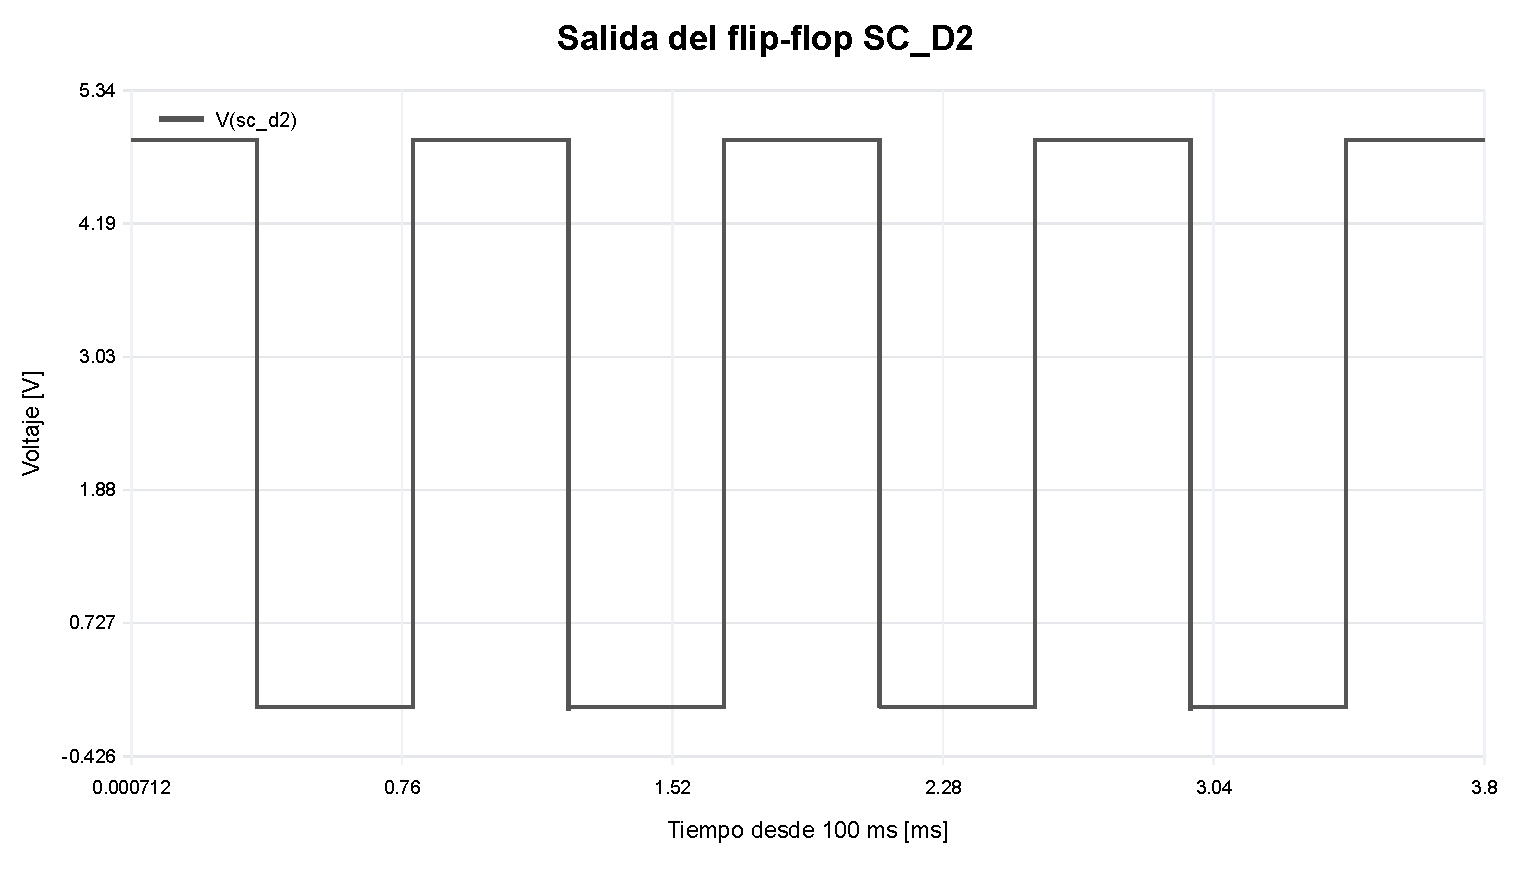
\includegraphics[width=0.88\linewidth]{figuras/integrado_sc_d2.pdf}
\caption{Salida dividida por dos \(SC\_D2\).}
\end{figure}

\begin{figure}[H]
\centering
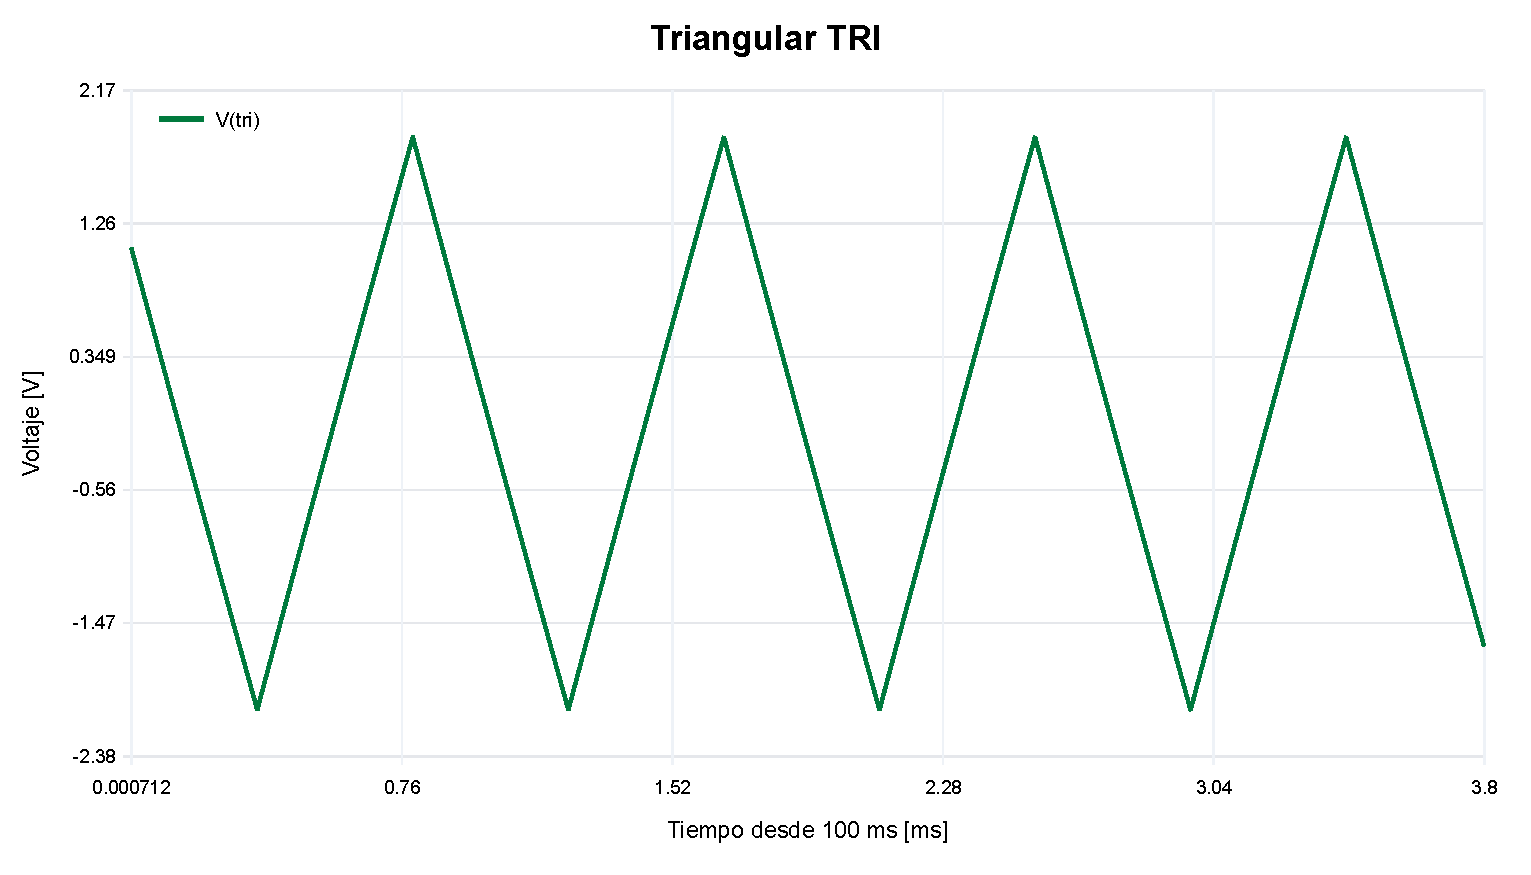
\includegraphics[width=0.88\linewidth]{figuras/integrado_tri.pdf}
\caption{Onda triangular \(TRI\).}
\end{figure}

\begin{figure}[H]
\centering
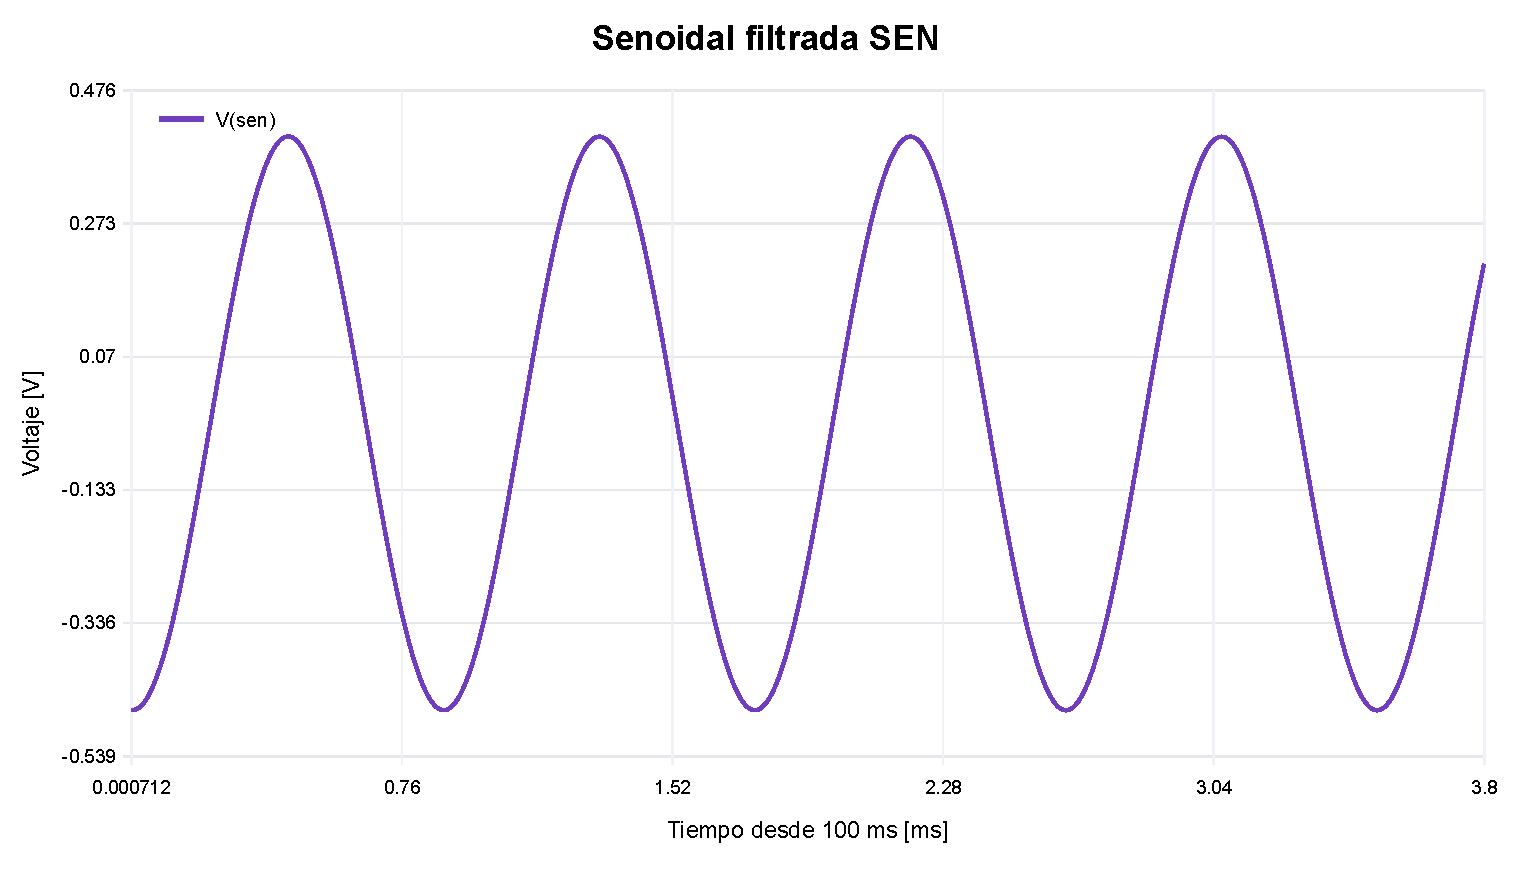
\includegraphics[width=0.88\linewidth]{figuras/integrado_sen.pdf}
\caption{Salida senoidal filtrada \(SEN\).}
\end{figure}

\section{Graficas de LTspice juntas}

La primera figura muestra todas las senales con su escala real. La segunda
figura usa normalizacion para comparar fase y forma de onda sin que la
amplitud de \(SC\) oculte las senales pequenas.

\begin{figure}[H]
\centering
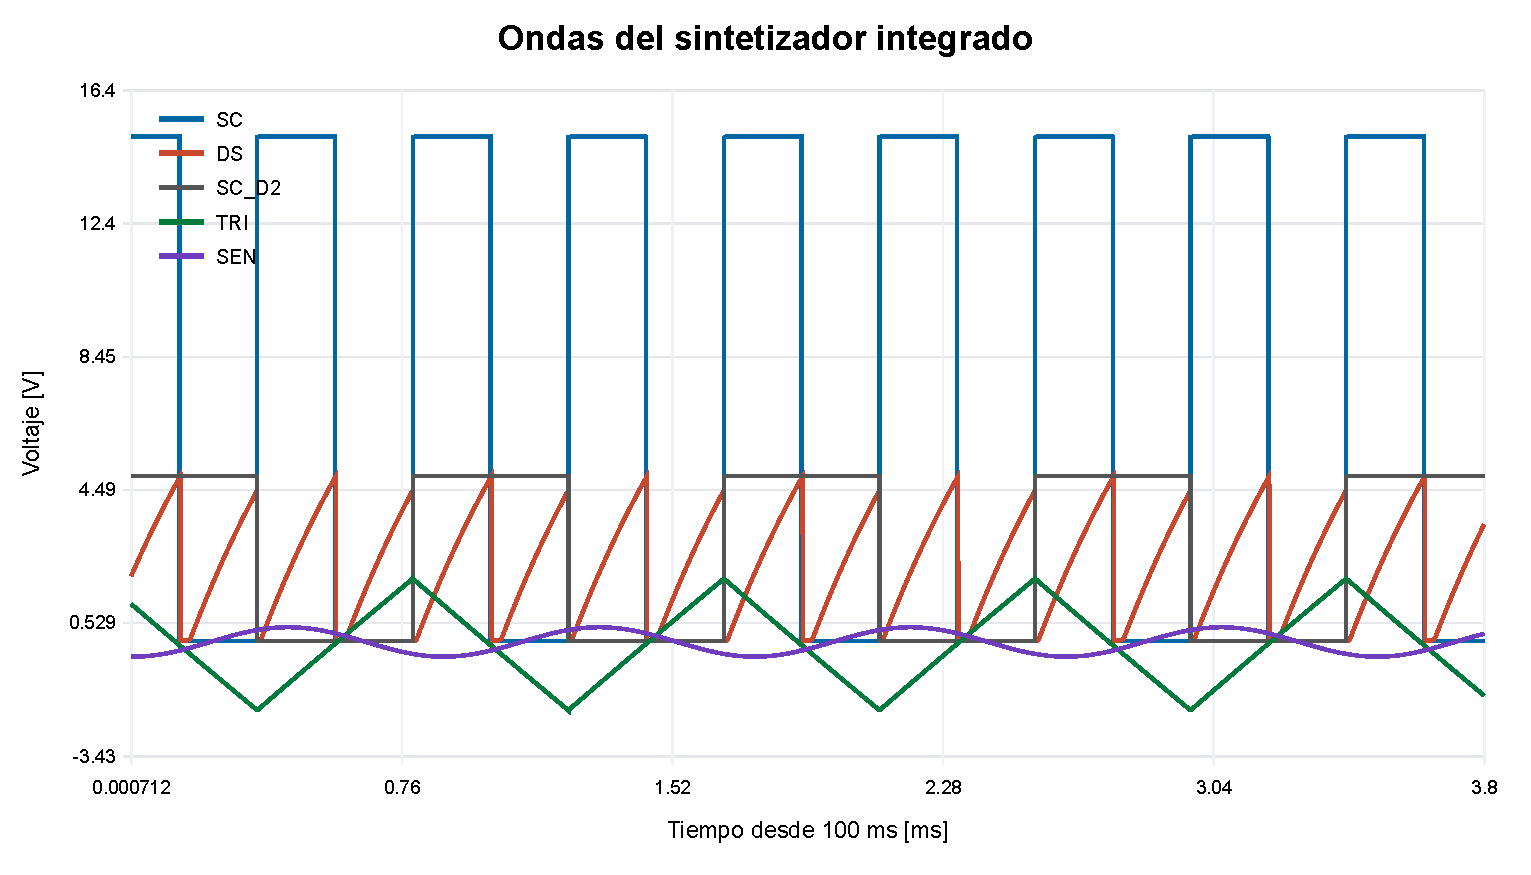
\includegraphics[width=0.92\linewidth]{figuras/integrado_ondas_juntas.pdf}
\caption{Ondas principales con escala real.}
\end{figure}

\begin{figure}[H]
\centering
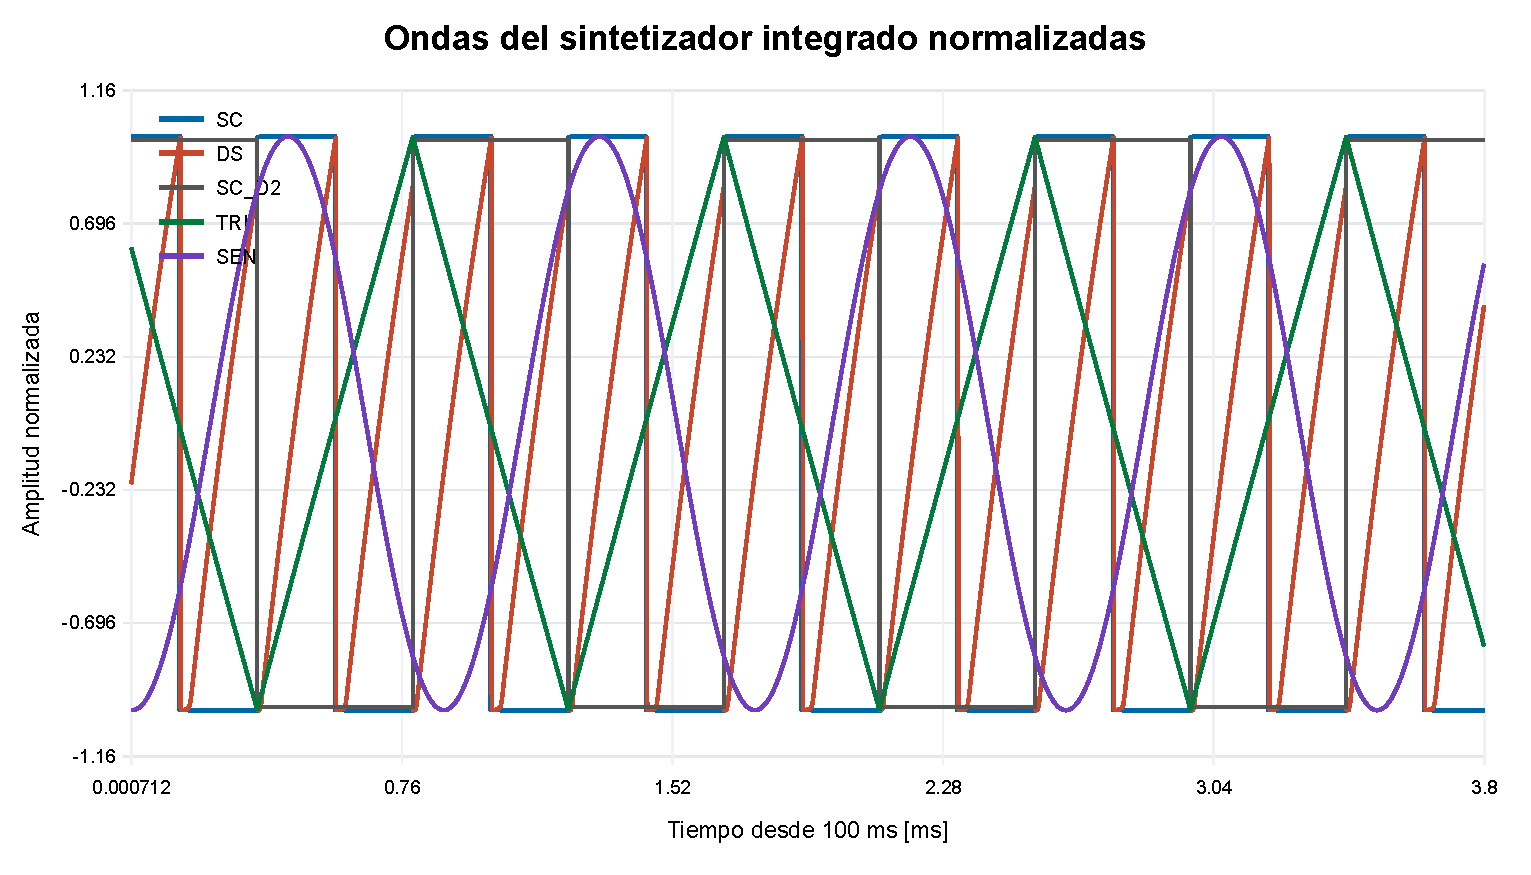
\includegraphics[width=0.92\linewidth]{figuras/integrado_ondas_juntas_normalizadas.pdf}
\caption{Ondas principales normalizadas.}
\end{figure}

\section{Archivos generados}

\begin{itemize}
  \item Documento fuente: \texttt{informe\_etapas\_sintetizador\_ltspice.tex}.
  \item Documento PDF: \texttt{informe\_etapas\_sintetizador\_ltspice.pdf}.
  \item Graficas: \texttt{figuras/integrado\_*.pdf} y
  \texttt{figuras/integrado\_*.svg}.
  \item Datos exportados: \texttt{datos/integrado\_*.csv}.
  \item Script de exportacion: \texttt{scripts/exportar\_graficas\_integrado.py}.
\end{itemize}

\section{Conclusion}

El sintetizador cumple las frecuencias objetivo del proyecto. La etapa con
\texttt{NE555} fija la frecuencia base, la etapa de transistores genera la
sierra a \(2f_0\), el flip-flop divide por dos para obtener \(f_0/2\), el
integrador produce la triangular y el filtro Chebyshev de quinto orden obtiene
la salida senoidal. La salida final medida en LTspice fue:

\[
\boxed{f_{SEN}=1144.8698~\text{Hz}}
\]

con un error de:

\[
\boxed{-0.0114\%}.
\]

\end{document}
